%\begin{figure}[h!]
%\centering
%\subfigure[]{
%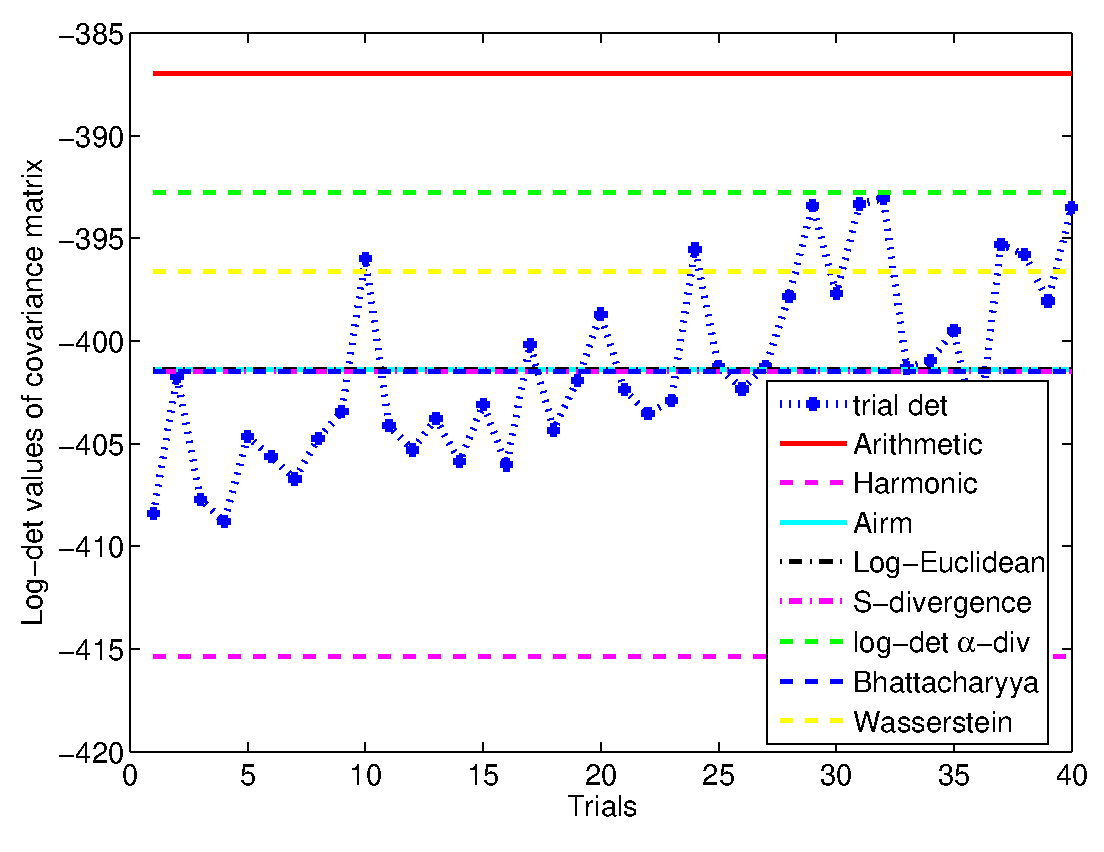
\includegraphics[width=0.46\textwidth]{figures/swel.eps}
%\label{fig:swel}
%}
%\subfigure[]{
%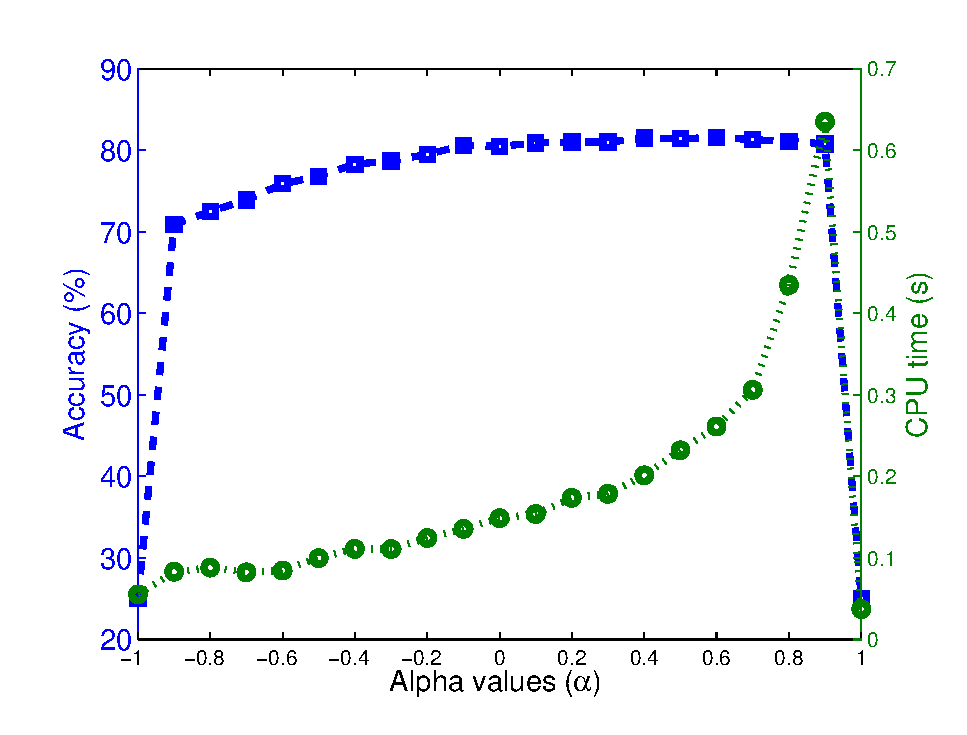
\includegraphics[width=0.49\textwidth]{figures/alpha_cross.eps}
%\label{fig:alphacross}
%}
%\caption{(a): Swelling effect of Arithmetic mean shown through log-determinant values. Training trials are taken from the 13Hz class of the subject with the highest BCI performance. Log-determinant values are given for each trial covariance (points), and for means of Table~\ref{tab:dist} (horizontal lines). (b): Classification accuracy and CPU time, obtained with $\alpha$-divergence for $-1\leqslant \alpha  \leqslant 1$.} 
%\label{fig:swel_alpha}
%\end{figure} 

\subsection{Results and discussion}

\iflatexml\else \changes{ \fi
Discuss the invariance to right- and left-multiplication by positive matrices. It brings a significant advantage over Euclidean metrics, in terms of electrode placement and unforseen displacement in electrodes position, and can even alleviate anatomical differences.
\iflatexml\else } \fi
%\begin{figure}[h!]
%\centering
%\subfigure[]{
%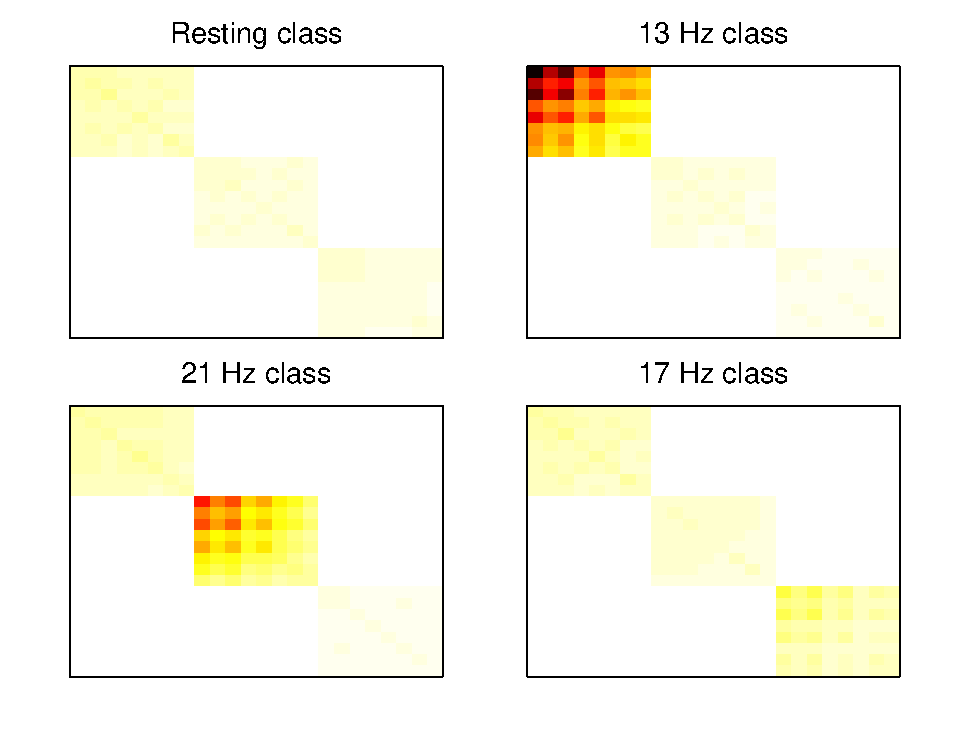
\includegraphics[width=0.47\textwidth]{Figures/covmat.eps}
%\label{fig:covmat12}}
%\subfigure[]{
%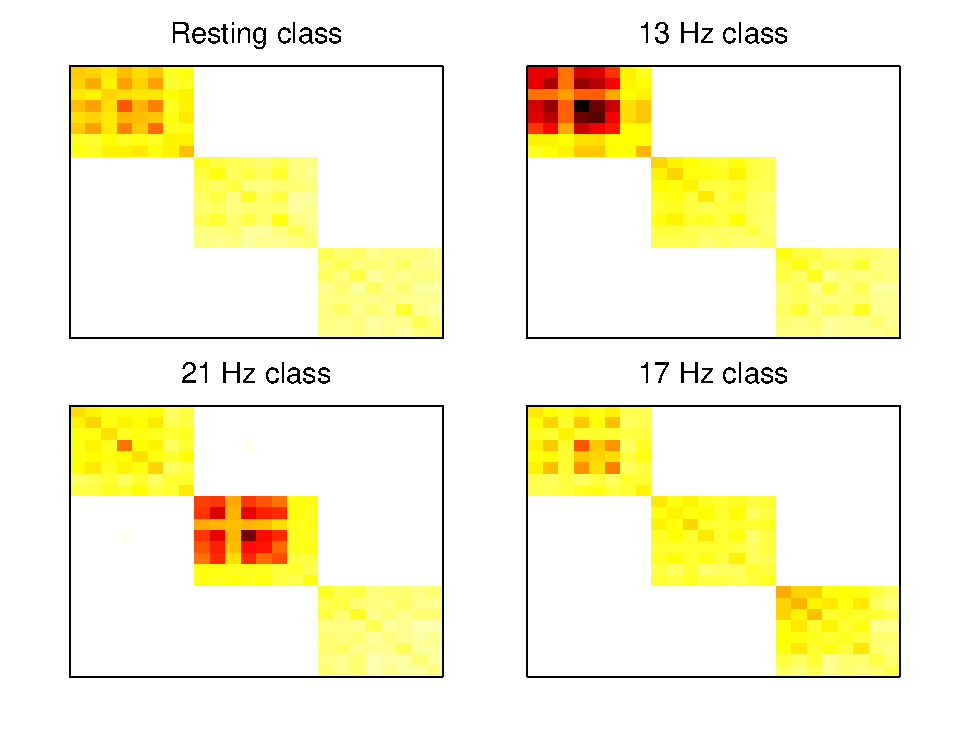
\includegraphics[width=0.47\textwidth]{Figures/covmat11.eps}
%\label{fig:covmat11}}
%\caption{Representation of covariance matrices: each image is the covariance matrix mean $\Pm^{(\ci)}$ of the class $\ci$, for one session of the recording. The diagonal blocks show the covariance in different frequency bands, i.e. 13Hz in the upper-left block, 21Hz in the middle, and 17Hz in the bottom-right. Subjects with highest (a) and lowest (b) BCI performance.}
%\label{fig:covmat}
%\end{figure}
